
%% bare_jrnl.tex
%% V1.4b
%% 2015/08/26
%% by Michael Shell
%% see http://www.michaelshell.org/
%% for current contact information.
%%
%% This is a skeleton file demonstrating the use of IEEEtran.cls
%% (requires IEEEtran.cls version 1.8b or later) with an IEEE
%% journal paper.
%%
%% Support sites:
%% http://www.michaelshell.org/tex/ieeetran/
%% http://www.ctan.org/pkg/ieeetran
%% and
%% http://www.ieee.org/

%%*************************************************************************
%% Legal Notice:
%% This code is offered as-is without any warranty either expressed or
%% implied; without even the implied warranty of MERCHANTABILITY or
%% FITNESS FOR A PARTICULAR PURPOSE! 
%% User assumes all risk.
%% In no event shall the IEEE or any contributor to this code be liable for
%% any damages or losses, including, but not limited to, incidental,
%% consequential, or any other damages, resulting from the use or misuse
%% of any information contained here.
%%
%% All comments are the opinions of their respective authors and are not
%% necessarily endorsed by the IEEE.
%%
%% This work is distributed under the LaTeX Project Public License (LPPL)
%% ( http://www.latex-project.org/ ) version 1.3, and may be freely used,
%% distributed and modified. A copy of the LPPL, version 1.3, is included
%% in the base LaTeX documentation of all distributions of LaTeX released
%% 2003/12/01 or later.
%% Retain all contribution notices and credits.
%% ** Modified files should be clearly indicated as such, including  **
%% ** renaming them and changing author support contact information. **
%%*************************************************************************


% *** Authors should verify (and, if needed, correct) their LaTeX system  ***
% *** with the testflow diagnostic prior to trusting their LaTeX platform ***
% *** with production work. The IEEE's font choices and paper sizes can   ***
% *** trigger bugs that do not appear when using other class files.       ***                          ***
% The testflow support page is at:
% http://www.michaelshell.org/tex/testflow/



\documentclass[journal]{IEEEtran}
%
% If IEEEtran.cls has not been installed into the LaTeX system files,
% manually specify the path to it like:
% \documentclass[journal]{../sty/IEEEtran}

% Some very useful LaTeX packages include:
% (uncomment the ones you want to load)


% *** MISC UTILITY PACKAGES ***
%
%\usepackage{ifpdf}
% Heiko Oberdiek's ifpdf.sty is very useful if you need conditional
% compilation based on whether the output is pdf or dvi.
% usage:
% \ifpdf
%   % pdf code
% \else
%   % dvi code
% \fi
% The latest version of ifpdf.sty can be obtained from:
% http://www.ctan.org/pkg/ifpdf
% Also, note that IEEEtran.cls V1.7 and later provides a builtin
% \ifCLASSINFOpdf conditional that works the same way.
% When switching from latex to pdflatex and vice-versa, the compiler may
% have to be run twice to clear warning/error messages.

% *** CITATION PACKAGES ***
%
%\usepackage{cite}
% cite.sty was written by Donald Arseneau
% V1.6 and later of IEEEtran pre-defines the format of the cite.sty package
% \cite{} output to follow that of the IEEE. Loading the cite package will
% result in citation numbers being automatically sorted and properly
% "compressed/ranged". e.g., [1], [9], [2], [7], [5], [6] without using
% cite.sty will become [1], [2], [5]--[7], [9] using cite.sty. cite.sty's
% \cite will automatically add leading space, if needed. Use cite.sty's
% noadjust option (cite.sty V3.8 and later) if you want to turn this off
% such as if a citation ever needs to be enclosed in parenthesis.
% cite.sty is already installed on most LaTeX systems. Be sure and use
% version 5.0 (2009-03-20) and later if using hyperref.sty.
% The latest version can be obtained at:
% http://www.ctan.org/pkg/cite
% The documentation is contained in the cite.sty file itself.


% *** GRAPHICS RELATED PACKAGES ***
%
\ifCLASSINFOpdf
  % \usepackage[pdftex]{graphicx}
  % declare the path(s) where your graphic files are
  % \graphicspath{{../pdf/}{../jpeg/}}
  % and their extensions so you won't have to specify these with
  % every instance of \includegraphics
  % \DeclareGraphicsExtensions{.pdf,.jpeg,.png}
\else
  % or other class option (dvipsone, dvipdf, if not using dvips). graphicx
  % will default to the driver specified in the system graphics.cfg if no
  % driver is specified.
  % \usepackage[dvips]{graphicx}
  % declare the path(s) where your graphic files are
  % \graphicspath{{../eps/}}
  % and their extensions so you won't have to specify these with
  % every instance of \includegraphics
  % \DeclareGraphicsExtensions{.eps}
\fi
% graphicx was written by David Carlisle and Sebastian Rahtz. It is
% required if you want graphics, photos, etc. graphicx.sty is already
% installed on most LaTeX systems. The latest version and documentation
% can be obtained at: 
% http://www.ctan.org/pkg/graphicx
% Another good source of documentation is "Using Imported Graphics in
% LaTeX2e" by Keith Reckdahl which can be found at:
% http://www.ctan.org/pkg/epslatex
%
% latex, and pdflatex in dvi mode, support graphics in encapsulated
% postscript (.eps) format. pdflatex in pdf mode supports graphics
% in .pdf, .jpeg, .png and .mps (metapost) formats. Users should ensure
% that all non-photo figures use a vector format (.eps, .pdf, .mps) and
% not a bitmapped formats (.jpeg, .png). The IEEE frowns on bitmapped formats
% which can result in "jaggedy"/blurry rendering of lines and letters as
% well as large increases in file sizes.
%
% You can find documentation about the pdfTeX application at:
% http://www.tug.org/applications/pdftex

% *** MATH PACKAGES ***
%
%\usepackage{amsmath}
% A popular package from the American Mathematical Society that provides
% many useful and powerful commands for dealing with mathematics.
%
% Note that the amsmath package sets \interdisplaylinepenalty to 10000
% thus preventing page breaks from occurring within multiline equations. Use:
%\interdisplaylinepenalty=2500
% after loading amsmath to restore such page breaks as IEEEtran.cls normally
% does. amsmath.sty is already installed on most LaTeX systems. The latest
% version and documentation can be obtained at:
% http://www.ctan.org/pkg/amsmath


% *** SPECIALIZED LIST PACKAGES ***
%
%\usepackage{algorithmic}
% algorithmic.sty was written by Peter Williams and Rogerio Brito.
% This package provides an algorithmic environment fo describing algorithms.
% You can use the algorithmic environment in-text or within a figure
% environment to provide for a floating algorithm. Do NOT use the algorithm
% floating environment provided by algorithm.sty (by the same authors) or
% algorithm2e.sty (by Christophe Fiorio) as the IEEE does not use dedicated
% algorithm float types and packages that provide these will not provide
% correct IEEE style captions. The latest version and documentation of
% algorithmic.sty can be obtained at:
% http://www.ctan.org/pkg/algorithms
% Also of interest may be the (relatively newer and more customizable)
% algorithmicx.sty package by Szasz Janos:
% http://www.ctan.org/pkg/algorithmicx




% *** ALIGNMENT PACKAGES ***
%
%\usepackage{array}
% Frank Mittelbach's and David Carlisle's array.sty patches and improves
% the standard LaTeX2e array and tabular environments to provide better
% appearance and additional user controls. As the default LaTeX2e table
% generation code is lacking to the point of almost being broken with
% respect to the quality of the end results, all users are strongly
% advised to use an enhanced (at the very least that provided by array.sty)
% set of table tools. array.sty is already installed on most systems. The
% latest version and documentation can be obtained at:
% http://www.ctan.org/pkg/array


% IEEEtran contains the IEEEeqnarray family of commands that can be used to
% generate multiline equations as well as matrices, tables, etc., of high
% quality.




% *** SUBFIGURE PACKAGES ***
%\ifCLASSOPTIONcompsoc
%  \usepackage[caption=false,font=normalsize,labelfont=sf,textfont=sf]{subfig}
%\else
%  \usepackage[caption=false,font=footnotesize]{subfig}
%\fi
% subfig.sty, written by Steven Douglas Cochran, is the modern replacement
% for subfigure.sty, the latter of which is no longer maintained and is
% incompatible with some LaTeX packages including fixltx2e. However,
% subfig.sty requires and automatically loads Axel Sommerfeldt's caption.sty
% which will override IEEEtran.cls' handling of captions and this will result
% in non-IEEE style figure/table captions. To prevent this problem, be sure
% and invoke subfig.sty's "caption=false" package option (available since
% subfig.sty version 1.3, 2005/06/28) as this is will preserve IEEEtran.cls
% handling of captions.
% Note that the Computer Society format requires a larger sans serif font
% than the serif footnote size font used in traditional IEEE formatting
% and thus the need to invoke different subfig.sty package options depending
% on whether compsoc mode has been enabled.
%
% The latest version and documentation of subfig.sty can be obtained at:
% http://www.ctan.org/pkg/subfig




% *** FLOAT PACKAGES ***
%
%\usepackage{fixltx2e}
% fixltx2e, the successor to the earlier fix2col.sty, was written by
% Frank Mittelbach and David Carlisle. This package corrects a few problems
% in the LaTeX2e kernel, the most notable of which is that in current
% LaTeX2e releases, the ordering of single and double column floats is not
% guaranteed to be preserved. Thus, an unpatched LaTeX2e can allow a
% single column figure to be placed prior to an earlier double column
% figure.
% Be aware that LaTeX2e kernels dated 2015 and later have fixltx2e.sty's
% corrections already built into the system in which case a warning will
% be issued if an attempt is made to load fixltx2e.sty as it is no longer
% needed.
% The latest version and documentation can be found at:
% http://www.ctan.org/pkg/fixltx2e


%\usepackage{stfloats}
% stfloats.sty was written by Sigitas Tolusis. This package gives LaTeX2e
% the ability to do double column floats at the bottom of the page as well
% as the top. (e.g., "\begin{figure*}[!b]" is not normally possible in
% LaTeX2e). It also provides a command:
%\fnbelowfloat
% to enable the placement of footnotes below bottom floats (the standard
% LaTeX2e kernel puts them above bottom floats). This is an invasive package
% which rewrites many portions of the LaTeX2e float routines. It may not work
% with other packages that modify the LaTeX2e float routines. The latest
% version and documentation can be obtained at:
% http://www.ctan.org/pkg/stfloats
% Do not use the stfloats baselinefloat ability as the IEEE does not allow
% \baselineskip to stretch. Authors submitting work to the IEEE should note
% that the IEEE rarely uses double column equations and that authors should try
% to avoid such use. Do not be tempted to use the cuted.sty or midfloat.sty
% packages (also by Sigitas Tolusis) as the IEEE does not format its papers in
% such ways.
% Do not attempt to use stfloats with fixltx2e as they are incompatible.
% Instead, use Morten Hogholm'a dblfloatfix which combines the features
% of both fixltx2e and stfloats:
%
% \usepackage{dblfloatfix}
% The latest version can be found at:
% http://www.ctan.org/pkg/dblfloatfix




%\ifCLASSOPTIONcaptionsoff
%  \usepackage[nomarkers]{endfloat}
% \let\MYoriglatexcaption\caption
% \renewcommand{\caption}[2][\relax]{\MYoriglatexcaption[#2]{#2}}
%\fi
% endfloat.sty was written by James Darrell McCauley, Jeff Goldberg and 
% Axel Sommerfeldt. This package may be useful when used in conjunction with 
% IEEEtran.cls'  captionsoff option. Some IEEE journals/societies require that
% submissions have lists of figures/tables at the end of the paper and that
% figures/tables without any captions are placed on a page by themselves at
% the end of the document. If needed, the draftcls IEEEtran class option or
% \CLASSINPUTbaselinestretch interface can be used to increase the line
% spacing as well. Be sure and use the nomarkers option of endfloat to
% prevent endfloat from "marking" where the figures would have been placed
% in the text. The two hack lines of code above are a slight modification of
% that suggested by in the endfloat docs (section 8.4.1) to ensure that
% the full captions always appear in the list of figures/tables - even if
% the user used the short optional argument of \caption[]{}.
% IEEE papers do not typically make use of \caption[]'s optional argument,
% so this should not be an issue. A similar trick can be used to disable
% captions of packages such as subfig.sty that lack options to turn off
% the subcaptions:
% For subfig.sty:
% \let\MYorigsubfloat\subfloat
% \renewcommand{\subfloat}[2][\relax]{\MYorigsubfloat[]{#2}}
% However, the above trick will not work if both optional arguments of
% the \subfloat command are used. Furthermore, there needs to be a
% description of each subfigure *somewhere* and endfloat does not add
% subfigure captions to its list of figures. Thus, the best approach is to
% avoid the use of subfigure captions (many IEEE journals avoid them anyway)
% and instead reference/explain all the subfigures within the main caption.
% The latest version of endfloat.sty and its documentation can obtained at:
% http://www.ctan.org/pkg/endfloat
%
% The IEEEtran \ifCLASSOPTIONcaptionsoff conditional can also be used
% later in the document, say, to conditionally put the References on a 
% page by themselves.




% *** PDF, URL AND HYPERLINK PACKAGES ***
%
\usepackage{url}
% url.sty was written by Donald Arseneau. It provides better support for
% handling and breaking URLs. url.sty is already installed on most LaTeX
% systems. The latest version and documentation can be obtained at:
% http://www.ctan.org/pkg/url
% Basically, \url{my_url_here}.
\usepackage{amsmath,amssymb,amsfonts}
\usepackage{algorithm,algorithmic}
\usepackage{graphicx}
\graphicspath{ {./images/} }
\usepackage{makecell}
\usepackage{textcomp}
\usepackage{xcolor}

% *** Do not adjust lengths that control margins, column widths, etc. ***
% *** Do not use packages that alter fonts (such as pslatex).         ***
% There should be no need to do such things with IEEEtran.cls V1.6 and later.
% (Unless specifically asked to do so by the journal or conference you plan
% to submit to, of course. )


% correct bad hyphenation here
\hyphenation{op-tical net-works semi-conduc-tor}


\begin{document}
%
% paper title
% Titles are generally capitalized except for words such as a, an, and, as,
% at, but, by, for, in, nor, of, on, or, the, to and up, which are usually
% not capitalized unless they are the first or last word of the title.
% Linebreaks \\ can be used within to get better formatting as desired.
% Do not put math or special symbols in the title.
%\title{An automated formal synthesis optimization method for sizing of stand-alone solar photovoltaic systems: case studies and comparative}
\title{Optimal Sizing of Stand-alone Solar PV Systems Through Automated Formal Synthesis Method}
%
%
% author names and IEEE memberships
% note positions of commas and nonbreaking spaces ( ~ ) LaTeX will not break
% a structure at a ~ so this keeps an author's name from being broken across
% two lines.
% use \thanks{} to gain access to the first footnote area
% a separate \thanks must be used for each paragraph as LaTeX2e's \thanks
% was not built to handle multiple paragraphs
%

\author{Alessandro~Trindade and Lucas~Cordeiro% <-this % stops a space
\thanks{A. Trindade is with the Department of Electricity, Federal University of Amazonas, Manaus, Brazil, e-mail: alessandrotrindade@ufam.edu.br.}% <-this % stops a space
\thanks{L. Cordeiro is with School of Computer Science, The University of Manchester, UK, e-mail: lucas.cordeiro@manchester.ac.uk.}% <-this % stops a space
\thanks{Manuscript received September XY, 2019; revised XXXXX 11, 2019.}}

% note the % following the last \IEEEmembership and also \thanks - 
% these prevent an unwanted space from occurring between the last author name
% and the end of the author line. i.e., if you had this:
% 
% \author{....lastname \thanks{...} \thanks{...} }
%                     ^------------^------------^----Do not want these spaces!
%
% a space would be appended to the last name and could cause every name on that
% line to be shifted left slightly. This is one of those "LaTeX things". For
% instance, "\textbf{A} \textbf{B}" will typeset as "A B" not "AB". To get
% "AB" then you have to do: "\textbf{A}\textbf{B}"
% \thanks is no different in this regard, so shield the last } of each \thanks
% that ends a line with a % and do not let a space in before the next \thanks.
% Spaces after \IEEEmembership other than the last one are OK (and needed) as
% you are supposed to have spaces between the names. For what it is worth,
% this is a minor point as most people would not even notice if the said evil
% space somehow managed to creep in.



% The paper headers
\markboth{IEEE Transactions on Sustainable Energy,~Vol.~XX, No.~YY, September~2019}%
{Trindade and Cordeiro: An automated formal synthesis optimization method for sizing of stand-alone solar photovoltaic systems}
% The only time the second header will appear is for the odd numbered pages
% after the title page when using the twoside option.
% 
% *** Note that you probably will NOT want to include the author's ***
% *** name in the headers of peer review papers.                   ***
% You can use \ifCLASSOPTIONpeerreview for conditional compilation here if
% you desire.




% If you want to put a publisher's ID mark on the page you can do it like
% this:
%\IEEEpubid{0000--0000/00\$00.00~\copyright~2015 IEEE}
% Remember, if you use this you must call \IEEEpubidadjcol in the second
% column for its text to clear the IEEEpubid mark.



% use for special paper notices
%\IEEEspecialpapernotice{(Invited Paper)}




% make the title area
\maketitle

% As a general rule, do not put math, special symbols or citations
% in the abstract or keywords.
\begin{abstract}
There exist various methods and computer tools to size solar photovoltaic systems; however, those tools are mainly based on simulations, which do not cover all aspects of the design-space during the search for the optimal solution. In prior studies related to optimal sizing of photovoltaic systems, the focus was always on criteria or objectives. Here, we present a novel sound and automated approach to obtain optimal sizing of stand-alone photovoltaic systems using an unprecedented program synthesis. In particular, our variant of counterexample guided inductive synthesis (CEGIS) approach has two phases: first we synthesize the sizing of stand-alone photovoltaic systems based on power reliability, but that may not achieve the lowest cost; second, the proposed solution is then verified iteratively with a lower bound cost via symbolic model checking. If the verification step does not fail, the lower bound is adjusted; and if it fails, a counterexample is provided with the optimal sizing, thereby linking the technical response of the first phase with cost analysis of the second phase. Commercial equipment data from different manufacturers are provided to our synthesis engine and candidate solutions are derived from financial analysis. Experimental results using seven case studies show that our synthesis method is able to produce within an acceptable run-time the optimal system sizing. We also present a comparative with a specialized simulation tool over real photovoltaic systems to show the effectiveness of our approach, which is able to provide more detailed and accurate solution than the existing simulation tool.
\end{abstract}

% Note that keywords are not normally used for peerreview papers.
\begin{IEEEkeywords}
Automated verification, model checking, program synthesis, electrical systems, solar photovoltaic systems.
\end{IEEEkeywords}


% For peer review papers, you can put extra information on the cover
% page as needed:
% \ifCLASSOPTIONpeerreview
% \begin{center} \bfseries EDICS Category: 3-BBND \end{center}
% \fi
%
% For peerreview papers, this IEEEtran command inserts a page break and
% creates the second title. It will be ignored for other modes.
\IEEEpeerreviewmaketitle



\section{Introduction}
% The very first letter is a 2 line initial drop letter followed
% by the rest of the first word in caps.
% 
% form to use if the first word consists of a single letter:
% \IEEEPARstart{A}{demo} file is ....
% 
% form to use if you need the single drop letter followed by
% normal text (unknown if ever used by the IEEE):
% \IEEEPARstart{A}{}demo file is ....
% 
% Some journals put the first two words in caps:
% \IEEEPARstart{T}{his demo} file is ....
% 
% Here we have the typical use of a "T" for an initial drop letter
% and "HIS" in caps to complete the first word.
%\IEEEPARstart{T}{his} demo file is intended to serve as a ``starter file''
%
%\IEEEPARstart{C}{yber}-Physical Systems (CPS) are engineered systems, which are built from, and depend upon, the seamless integration of computational and physical  components~\cite{NSF2015}. During operation, such components must frequently adapt to the operating environment changes faced at run-time (dynamics of the physical processes) and must be able to continue to behave in a controlled and safe way, thus posing novel technical challenges for the software engineering of services and applications for CPS~\cite{Metzger2014}. Software pervasiveness in CPS places new challenges; in particular, highly dynamic environments, rapidly changing requirements, unpredictable and uncertain operating conditions demand new paradigms for software design~\cite{Filieri2015}.
%
%While some research efforts do exist to enhance and optimize the software development processes for CPS, further investigation and discussion of better and more effective models are still needed in practice~\cite{Al-Jaroodi2016}. Among the opportunities for enhancements in the software development processes for CPS, there exists the need for developing new techniques and tools to support CPS requirements gathering and analysis with the goal of synthesizing \textit{correct-by-construction} implementations of CPS. These techniques need to deal with predefined requirements enforced by the nature and inherited constraints of the target CPS. In addition, they should be able to provide verification and validation mechanisms for completeness, correctness, and consistency~\cite{Al-Jaroodi2016}. Uncertainty and variability, at the same time, can be dealt with formal verification~\cite{NESSI}. Energy production, distribution, and optimization are all CPS problems~\cite{UC}. 

\IEEEPARstart{L}{ack} of access to clean and affordable energy is considered a core dimension of poverty~\cite{Hussein2012}. Progress has been made worldwide; in particular, the number of people without electricity access fell below $1$ billion threshold for the first time in $2017$~\cite{IEAweo2018}. In order to provide universal electricity for all, decentralized systems led by solar photovoltaic (PV) in off-grid and mini-grid systems will be the lowest-cost solution for three-quarters of the additional connections needed~\cite{Hussein2012}; specifically grid extension will be the standard in urban areas~\cite{IEAweo2018}.

In order to simulate or evaluate a PV system, there exist various specialized tools, e.g., RETScreen, HOMER, PVWatts, SAM and Hybrid2~\cite{Pradhan,Swarnkar,NRELDobos,NRELBlair,Mills}; and even general purpose simulation tools, e.g.,  PSpice~\cite{Gow1999}, or MATLAB/Simulink package~\cite{Benatiallah2017}. However, these tools are based on simulation; they have the drawback of an incomplete coverage  since verification of all possible combinations and potential failures of a system is unfeasible~\cite{ClarkeHV18}. 

Optimization of PV systems is not a recent topic; since the $90$'s different techniques using a wide variety of criteria to find ultimate combinations for design parameters, based on intuitive, numerical and analytical methods were developed and evaluated~\cite{Applasamy2011}. An ideal combination of any PV system is made by the best compromise between two considered objectives, which is power \textit{reliability} and \textit{system cost}~\cite{Alsadi2018}.

Formal methods could offer a great potential to obtain a more effective design process to PV systems~\cite{ClarkeHV18}. Related to past studies where formal methods are applied to the energy area, in $2012$, a Chinese smart grid implementation was considered as case study to address the verification problem for performance and energy consumption~\cite{Yukseletall2012}. In $2015$, automated simulation-based verification technique was applied to verify correctness of power system protection settings ~\cite{Sengupta2015}. In $2017$, a researcher suggested the application of formal methods to verify and control the behavior of computational devices, interacting over a smart grid  infrastructure~\cite{Abate2017}. Finally, in $2018$, a verification methodology was applied to PV panels (not a complete PV system) and its distributed power point tracking~\cite{Driouich2018}. However, past studies did not deal with electricity generation or even solar PV systems optimization. Formal methods based on \textit{symbolic model checking} and its application to synthesize PV systems have not been further explored in literature.
 
Here, we have developed a variant of counterexample guided inductive synthesis (CEGIS) for synthesizing optimal sizing of stand-alone PV systems using commercial equipment data. Given a correctness specification $\sigma$, our method uses that as starting point and then iteratively produces a sequence of candidate solutions that satisfy $\sigma$, related to power reliability. In particular, in each iteration, we synthesize sizing of stand-alone PV systems but that may not achieve the lowest cost. The candidate solution is then verified via symbolic model checking with a lower bound that serves as the minimum cost of reference; if the verification step does not fail, the lower bound is adjusted. If it fails then a counterexample is provided with an optimal sizing that meets power reliability and system cost. Note that in this study, our focus is not on a novel criteria or even optimization objectives. Instead, our novelty relies on an effective approach on the pursuit of the optimal solution of PV systems using formal methods. %, which outperforms existing state-of-the-art simulation tool.

%Our work makes two major contributions. \textbf{First}, the use of automated symbolic verification methods in electrical systems was rare in recent prior studies~\cite{abs-1811-09438}, and specifically their use in synthesizing optimal PV sizing is unprecedented. Here, a list of PV components (i.e., PV panels, charge controllers, inverters, and batteries) can be fed to our proposed synthesis method together with user requirements and environment constraints, and our synthesis algorithm based on symbolic model checking can find the optimal solution in technical and economical terms. \textbf{Second}, %our experimental results show that our synthesis method is an effective and efficient approach on the pursuit of the optimal solution of PV systems using formal methods, which outperforms existing state-of-the-art simulation tool. As a result, 
\textit{Contribution}. Our study marks the first application of a sound and automated formal synthesis approach able to provide accurate results of optimal sizing of stand-alone PV systems, which outperforms existing state-of-the-art simulation tool used in a comparative with seven case studies. Thus, we considerably advance the state-of-the-art in applied energy over the last two decades with the goal of optimally designing PV systems.

\textit{Outline}. Section~\ref{sec:Background} gives the background about sizing and optimization of PV systems. Section~\ref{sec:Method} presents the automated formal synthesis proposed in this underlying study. Section~\ref{sec:Results} is devoted to the experimentation, results and analysis. Section~\ref{sec:Conclusion} presents the conclusion and describes future work.

\section{Sizing and Optimization of PV Systems}
\label{sec:Background}
%-----------------------------------------------------------

A stand-alone PV system block diagram is illustrated in Fig.\ref{fig:blockdiagram}. %It identifies the PV generator, batteries, charge controller, inverter, and AC load. 
The PV generator (a panel or an array) is a semiconductor device that can convert solar energy into DC electricity. For night hours or rainy days, we hold batteries where power can be stored and used. The use of batteries as a storage form implies the presence of a charge controller~\cite{Hansen}. The PV arrays produce DC and therefore when the PV system contains an AC load, a DC/AC conversion (inverter) is required. The AC load dictates the behavior of AC electrical load from the house. % that will be fed by the PV system.

\begin{figure}[h]
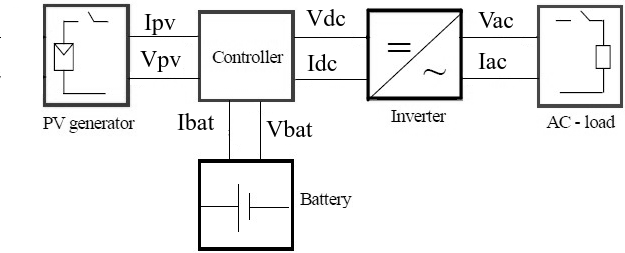
\includegraphics[width=0.4\textwidth]{blockdiagramPVS2_rev}
\centering
\caption{Block diagram for a typical stand-alone PV system~\cite{Hansen}.}
\label{fig:blockdiagram} 
\end{figure}

In this section we explain the adopted method to size stand-alone solar PV systems, and what criteria and technique is possible to apply for the optimal sizing. 

%%%%%%%%%%%%%%%%%%%%%%%%%%%%%%%%%%%%%%%%%%%%%%%%%%%%%%%%
\subsection{Sizing Stand-alone Solar PV Systems}
\label{sec:sizing}
%%%%%%%%%%%%%%%%%%%%%%%%%%%%%%%%%%%%%%%%%%%%%%%%%%%%%%%%

At this work, was adopted the critical period solar energy method~\cite{Pinho}, and MPPT (Maximum Power Point Tracking) charge controller (which is the most common nowadays). Firstly, we need to correct the energy consumption estimated to the load ($E_{consumption}$), which is carried out by Eq.~\eqref{eq:Ecorrected}, where the efficiency of batteries ($\eta_{b}$), controller ($\eta_{c}$), and inverter ($\eta_{i}$) are considered~\cite{Pinho} as follows

\begin{equation}
\label{eq:Ecorrected}
E_{corrected} = \dfrac{E_{consumption}}{\eta_{b} \eta_{c} \eta_{i} }.
\end{equation}

We also need to estimate the energy that can be produced for each panel, called $E_{p}$, in Wh, defined as

\begin{equation}
\label{eq:Ep}
E_{p} = Solar\_Irradiance \times Panel\_Area \times \eta_{p} \times 1000,
\end{equation}

\noindent where the solar irradiance is expressed in terms of $kWh/m^{2}$ and depends on the site where the PV system will be deployed; 
the PV panel area is given in $m^{2}$ and corresponds to the size of one PV panel, and $\eta_{p}$ represents the PV panel efficiency.
The total minimum number of needed solar panels ($N_{TPmin}$) is computed as

\begin{equation}
\label{eq:NTPmin}
N_{TPmin} = \dfrac{E_{corrected}}{E_{p}}.
\end{equation}

Particularly, the total number of panels in series ($N_{PSmin}$) and parallel ($N_{PPmin}$) are respectively given by

\begin{equation}
\label{eq:NPSmin}
\dfrac{V_{mppt,min}}{V_{maxPower,TempMax}} \leq N_{PSmin} \leq \dfrac{V_{mppt,max}}{V_{maxPower,TempMin}},
\end{equation}

\begin{equation}
\label{eq:NPPmin}
N_{PPmin} = \dfrac{P_{total}}{Number\,Panels\,Series \times P_{max,ref}},
\end{equation}

\noindent where $V_{mppt,max}$ is the maximum operation voltage and $V_{mppt,min}$ 
is the minimum operation voltage of the charge controller; $V_{maxPower,TempMax}$ and 
$V_{maxPower,TempMin}$ are the maximum power voltage from the PV module considering 
the maximum and minimum operational temperature, respectively; 
$P_{total}$ is the total power demanded from the PV system and 
$P_{max,ref}$ is the power supplied from one PV panel in $Watts$.
Regarding batteries, we must first define the total capacity of the battery bank, which can be described as

\begin{equation}
\label{eq:Cbank}
C_{bank} = \dfrac{E_{corrected} \times autonomy}{V_{system} \times DOD},
\end{equation}

\noindent where the variable $autonomy$ is a design definition and normally has a value ranging from $6$ to $48$h; 
$ V_{system} $ is the DC voltage of the bus, and $ DOD $ is the battery deep of discharge (considered of maximum of 25\% here).

Secondly, the total (minimum) number of batteries is computed as 

\begin{equation}
\label{eq:Nbtotal}
N_{B}total = N_{BS}min \times N_{BP}min
\end{equation}

\begin{equation}
\label{eq:Nbtotal2}
N_{B}total = \dfrac{V_{system}}{V_{bat}} \times \dfrac{C_{bank}}{1 \,Battery \, Capacity}.
\end{equation}

Regarding the charge controller, it must initially meet the voltage requirement of the PV system, as described by Eq.~\eqref{eq:vcvsystem} to the charge controller voltage: 

\begin{equation}
\label{eq:vcvsystem}
V_{c} = V_{system}.
\end{equation}

The short circuit reference information from the manufacturer's solar panel must be corrected 
to the cell temperature because the field temperature is higher than the nominal or laboratory temperature, and PV system is temperature dependent, as 

\begin{equation}
\label{eq:iscamb}
I_{sc,amb} = \dfrac{G}{G_{ref}} \left[ I_{sc,ref} + \mu_{I} \times (T-25) \right]. 
\end{equation}

The controller must meet the maximum current from the PV array given by Eqs.~\eqref{eq:icmin} and~\eqref{eq:icicmin} as

\begin{equation}
\label{eq:icmin}
I_{c,min} = I_{sc,amb} \times N_{PP},
\end{equation}

\begin{equation}
\label{eq:icicmin}
I_{c} \geq I_{c,min}.
\end{equation}

The inverter sizing check is performed by means of three equations. Eq.~\eqref{eq:vindc} ensures that 
the input voltage of the controller meets the system voltage. Eq.~\eqref{eq:voutac} ensures that the 
output voltage of the controller meets the AC voltage of the load. Finally, Eq.~\eqref{eq:invcheck} ensures that 
the controller can support the total demand of the load ($Demand$) and the surge power ($P_{surge}$), 
where $V_{in}DC$ is the nominal input voltage and $V_{out}AC$ is the nominal output voltage of the inverter; 
$MAX_{AC,ref}$ is the peak power that the inverter can support.

\begin{equation}
\label{eq:vindc} 
V_{in}DC = V_{system}.
\end{equation}

\begin{equation}
\label{eq:voutac} 
V_{out}AC = V_{AC}.
\end{equation}

\begin{equation}
\label{eq:invcheck} 
\left[ (Demand \leq P_{AC,ref}) \, and \, (P_{surge} \leq MAX_{AC,ref}) \right].
\end{equation}

%%%%%%%%%%%%%%%%%%%%%%%%%%%%%%%%%
\subsection{PV Systems Optimization: Criteria and Techniques}
%%%%%%%%%%%%%%%%%%%%%%%%%%%%%%%%%

In order to select an optimal PV system to meet sizing constraints, it is necessary to evaluate power reliability and system cost analysis for the underlying system. An ideal combination of any PV system is made by the best compromise between these two objectives or \textbf{criteria}.

During the PV system design, one of the most important aspects to ensure power system reliability is to analyze power supply availability~\cite{Alsadi2018}. The reason is because solar energy production is intermittent and, therefore, the energy generated usually will not match with the load demand. A reliable power is a generation system that has sufficient power to feed load demand in a period. There exist different methods to express system reliability, where the most popular ones are the loss of load probability (LOLP) and the loss of power supply probability (LPSP)~\cite{Alsadi2018}. In both methods, if the probability is zero, then the load will always be fulfilled; otherwise (i.e., probability of one) the load will never be fulfilled. LOLP is the probability for the case when a load demand exceeds the generation power by the PV system. On one hand, we claim that we have a reliable PV system when it is able to generate sufficient power to fulfill the demanded load within a time span. On the other hand, LPSP is defined as the probability of the case when system generates insufficient power to satisfy the load demand. The main approaches to LPSP demand simulation or probabilistic treatment of time series data to predict dynamic changing on system performance. However, data is not always available and dynamic analysis is complex; and this is a drawback of LOLP and LPSP~\cite{Alsadi2018}.

Related to economic analysis, there exist various methods available. The main objective is to determine whether the project has an acceptable investment; the usual way is to perform economic analysis after reliability analysis with the goal of proposing a system with high reliability and lowest cost~\cite{Alsadi2018}. The common methods include: Net Present Cost (NPC)~\cite{Park2004}, the Levelized Cost of Energy (LCOE)~\cite{Zhou2010}, or the Life Cycle Cost (LCC)~\cite{Applasamy2011}. The NPC is the present value of all the costs over the project lifetime, minus the present value of all the revenues that it earns over the project lifetime. The net present worth is found by discounting all cash inflows and outflows, including cost of installation, replacement and maintenance of the PV system, at an internal rate of return (IRR)~\cite{Park2004}. IRR is used to evaluate the attractiveness of a project or investment. LCOE is defined as the average cost per kWh of useful electrical energy produced by the PV system when a lifetime, investment cost, replacement, operation and maintenance, and capital cost are considered~\cite{Kamel2005}. LCOE method is useful in comparing different generation technologies with different operating characteristics~\cite{Zhou2010}. LCC is the estimation of sum of installation cost, operating and maintenance of a PV system for a period of time, and expressed in today's value~\cite{Applasamy2011}. Eq.~\eqref{eq:LCC} is used to calculate LCC of a PV system,

\begin{equation}
\label{eq:LCC}
\begin{aligned}
LCC = & C_{PV} + C_{bat} + C_{charger} + C_{inv} + \\
      & C_{installation} + C_{batrep} + C_{PWO\&M},
\end{aligned}
\end{equation}

\noindent where $C_{PV}$ is PV array cost, $C_{bat}$ is initial cost of batteries, $C_{charger}$ is cost of charger, $C_{inv}$ is inverter cost, $C_{installation}$ is installation cost, $C_{batrep}$ is battery replacement cost in present value, and $C_{PWO\&M}$ is operation and maintenance costs 
in present worth.

Parallel to criteria, in order to recommend an optimal configuration for PV systems, 
the designer has to evaluate the design based on optimization variables. 
As the number of optimization variables increases, the computational effort 
will increase as well. Hence, to obtain the best PV system design as well as 
simplified sizing process, prior work introduced three main \textbf{techniques} 
for system sizing calculation, namely intuitive, numerical, and analytical methods~\cite{Zhou2010}. Intuitive method is simple, easy to be implemented, and can be used to give rough suggestion for preliminary design. The sizing rules are based on designer's experience, using lowest performance either in a time period data or by directly using average value (daily, monthly, or annual) of solar irradiance. This method does not consider the battery's state of charge, or even the random nature of solar irradiation and meteorological conditions~\cite{Alsadi2018}. For numerical method, the design is simulated for each time step within a period. State of charge of batteries is calculated and investigated. It is very accurate, however is complex, demanding more time for calculation~\cite{Park2004}. Analytical methods is used to obtain a close relation or correlation in a form of equation between capacities and reliabilities. The sizing task becomes much simpler than numerical technique; however, the relation cannot be applied to different sites since it is specific to one place of deployment of the PV system, 
thereby demanding adaptation if another site is analyzed.

%------------------------------------------------------
\section{Automated Formal Synthesis Method}
\label{sec:Method}
%------------------------------------------------------

In this section we present the theory and the methodology created to obtain the optimal sizing of stand-alone solar PV systems through program synthesis.

\subsection{Automated Verification Using Model Checking}
\label{sec:AutomatedVerification}
%%%%%%%%%%%%%%%%%%%%%%%%%%%%%%%%%%

Although simulation and testing explore possible behaviors and scenarios of a given system, 
they leave open the question of whether unexplored trajectories may contain a flaw. 
Formal verification conducts an exhaustive exploration of all possible behaviors; 
when a design is said to be ``correct'' by a formal verification method, it implies that all 
behaviors have been explored, and questions regarding adequate coverage or missed behavior 
becomes irrelevant~\cite{Clarke2012}. Formal verification is a systematic approach that 
applies mathematical reasoning to obtain guarantees about the correctness of a system; 
one successful method in this domain is model checking~\cite{Clarke2012}. 

In order to perform the automated formal synthesis, we will use a state-of-the-art model checker, who was awarded with the Golden Medal at the annual competition in software verification~\cite{LMU2019}, the \textbf{CPAchecker}.

Automatic program verification requires a choice between precision and efficiency. 
The more precise a method, the fewer false positives it will produce, but also the 
more expensive it is, and thus applicable to fewer programs. 
Historically, this trade-off was reflected in two major approaches to static verification: 
program analysis and model checking. In order to experiment with the trade-off, 
and in order to be able to set the dial between the two extreme points, 
Configurable Program Analysis (CPA) provides a conceptual basis for expressing 
different verification approaches in the same formal setting. The CPA formalism 
provides an interface for the definition of program analyses. Consequently, CPAchecker provides an implementation framework that allows the seamless integration of program analyses that are expressed in the CPA framework. Related to the architecture, the central data structure is a set of control-flow automata (CFA), which consists of control-flow locations and control-flow edges. The CPA framework provides interfaces to SMT (Satisfiability Modulo Theories) solvers and interpolation procedures~\cite{Beyer2011}. Currently, CPAchecker uses MathSAT as SMT solver~\cite{Beyer2011}. 

%-----------------------------------------------------------
\subsection{Program Synthesis Technique}
\label{sec:ProgramSynthesis}
%-----------------------------------------------------------

Program synthesis addresses an age-old problem in computer science: can a computer program itself?~\cite{Bornholt2019}. Before the computer can automatically generate a program, it is necessary to give it a specification of what the program should do. The specification needs to describe the program’s desired behavior in order to ensure that the program does what it is intended.

Therefore, the basic idea of program synthesis is to automatically construct a program $P$ that satisfies a correctness specification $\sigma$. In particular, program synthesis is automatically performed by engines that use a correctness specification $\sigma$, as starting point, and then incrementally produce a sequence of candidate solutions that partially satisfy $\sigma$~\cite{Abateetal2017}. As a result, a given candidate program $p$ is iteratively refined, in order to match $\sigma$ more closely. CEGIS represents one of the most popular approaches to program synthesis that are currently used in practice for cyber-physical problems~\cite{Abateetal2017}, as energy production, distribution, and optimization, and  whose basic architecture is illustrated in Figure~\ref{Counter-Example-Guided-Inductive-Synthesis} and has close connections to algorithmic debugging using counterexamples and abstraction refinement~\cite{Alur} from model checking. 

\begin{figure}[h]
	\centering
	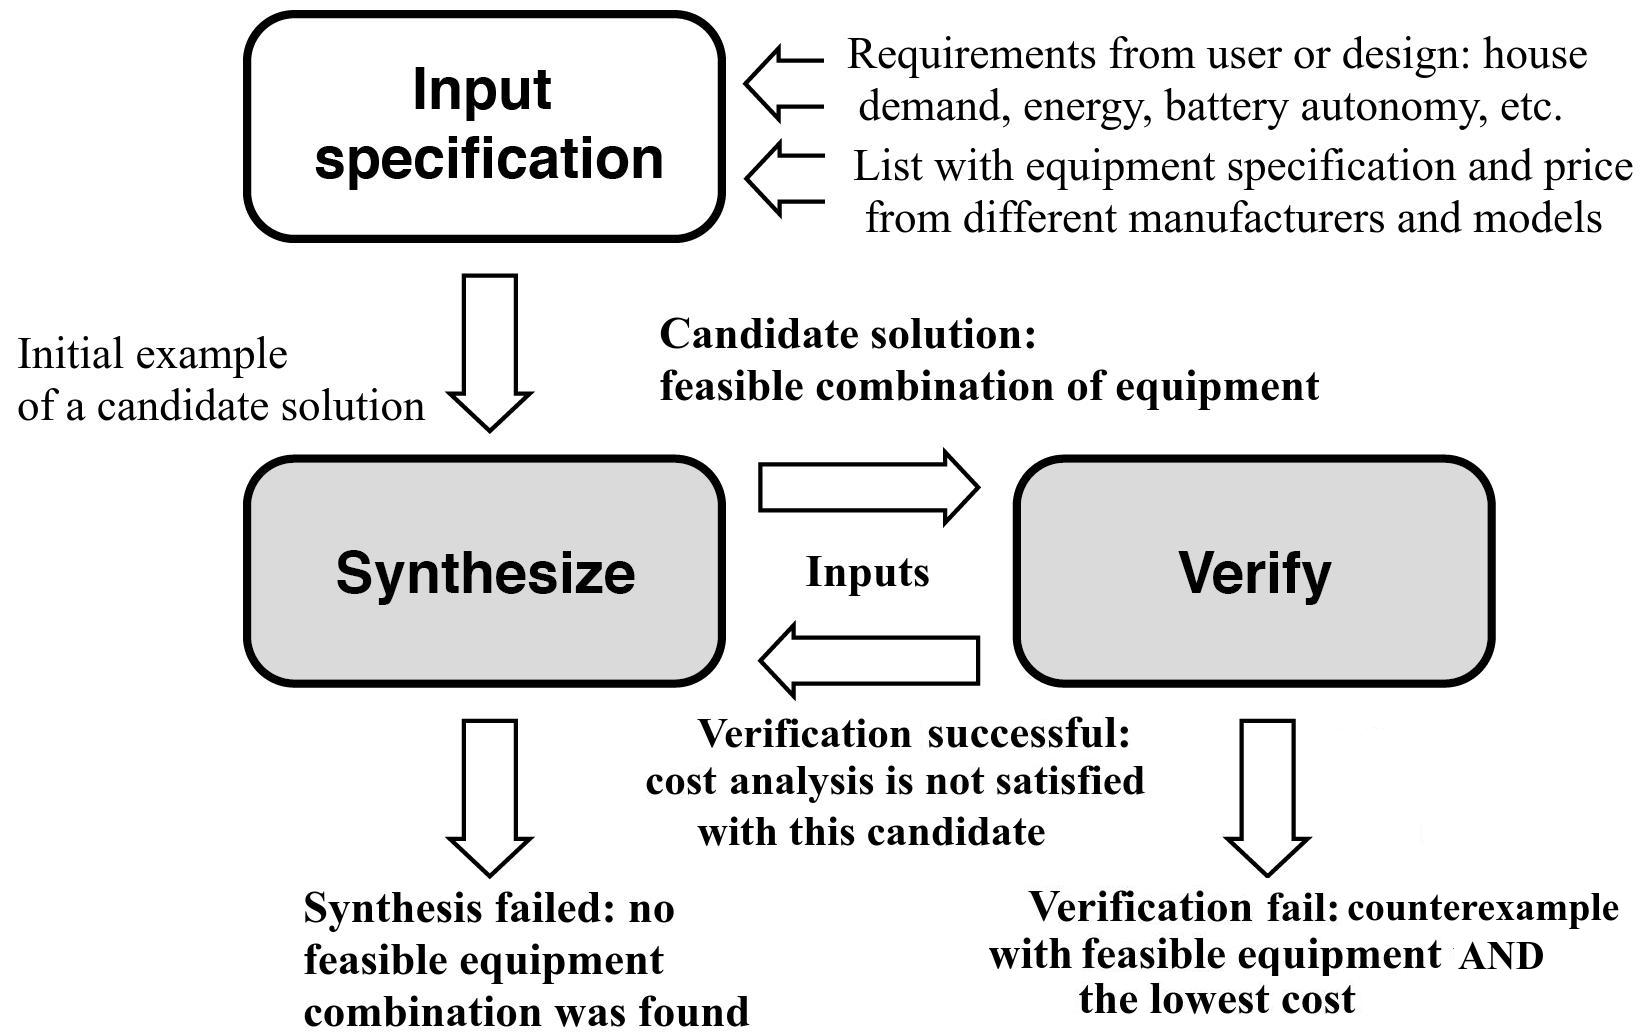
\includegraphics[width=0.75\columnwidth]{fig2_rev2.jpg}
	\caption{CEGIS applied to PV system sizing.}
	\label{Counter-Example-Guided-Inductive-Synthesis}
\end{figure}

The correctness specification $\sigma$ provided to our program synthesizer is of the form $\exists \vec{F} .  \forall \vec{x}.  \sigma(\vec{x}, \vec{F})$, where $\vec{F}$ ranges over functions, $\vec{x}$ ranges over ground terms, and $\sigma$ is a quantifier-free (QF) formula typically supported by SMT solvers. The ground terms are interpreted over some finite domain $\mathcal{D}$, where $\mathcal{D}$ can be encoded using the SMT's bit-vectors part. Examples of specification used by our method include house demand, energy, and battery autonomy; we also provide a list of equipment specification and price from different manufacturers and models.

In Figure~\ref{Counter-Example-Guided-Inductive-Synthesis}, regarding traditional CEGIS method, the phases {\sc Synthesize} and {\sc Verify} interact via a finite set of test vectors {\sc inputs}, which is incrementally updated. Given the correctness specification $\sigma$, the {\sc Synthesize} procedure tries to find an existential witness $\vec{F}$ satisfying the specification $\sigma(\vec{x}, \vec{F})$, for all $\vec{x}$ in {\sc inputs} (as opposed to all $\vec{x} \in \mathcal{D}$). If {\sc Synthesize} succeeds in finding a witness~$\vec{F}$, the latter is a candidate solution (i.e., feasible combination of equipment) to the full synthesis formula, which is passed to {\sc Verify} in order to check whether it is a proper solution ({\it i.e.}, $\vec{F}$ satisfies the specification $\sigma(\vec{x}, \vec{F})$ for all $\vec{x}\in\mathcal{D}$). If this is the case, then the algorithm terminates, i.e., we have found a feasible equipment with the lowest cost; otherwise, in the CEGIS traditional method, additional information is provided to the phase {\sc Synthesize}, in the form of a new counterexample that is added to the {\sc inputs} set and the loop iterates again.

One may notice that each iteration of the traditional CEGIS loop adds a new input to the finite set $\text{\sc inputs}$, which is then used for synthesis.  Given that the full set of inputs $\mathcal{D}$ is finite because we use bit-vector expressions, this means that the refinement loop can only iterate over a finite number of times; however, {\sc Synthesize} may conclude that no candidate solution obeying $\sigma$ for the finite set $\text{\sc inputs}$ exists and our synthesis engine can then conclude that no feasible equipment combination was found.

However, in our variant CEGIS method proposed here, there are four particular differences related to the traditional CEGIS: 
(1) there exists no test vector and every candidate is generated during the run-time in the {\sc Synthesize} phase and sent to the {\sc Verify} phase; 
(2) if the {\sc Verify} phase is unsuccessful, then a new candidate is generated by {\sc Synthesize} and 
(3) the lower bound of the {\sc Verify} phase is incremented to search for the lowest cost; 
(4) as a result, there exists no refinement from the {\sc Verify} phase back to the {\sc Synthesize} phase, i.e., 
a new counterexample is not added to the {\sc input} set since a failure during the {\sc Verify} phase will only discard 
a given candidate that could be feasible in the next iteration with a new lower bound.

Program synthesis engines that implement the CEGIS approach~\cite{sketch} can automatically produce solutions for a large variety of specifications; here we have used symbolic software verifiers based on SMT solvers.

Algorithm~\ref{alg:verification-algorithm} describes our pseudo-code to synthesize stand-alone PV systems using symbolic model checking. It was adopted the analytical method of optimization, with LCC economical analysis and power reliability based on the critical period criteria.

 \begin{algorithm}
 \caption{Synthesis algorithm}
 \begin{algorithmic}[1]
 \renewcommand{\algorithmicrequire}{\textbf{Input:}}
 \renewcommand{\algorithmicensure}{\textbf{Output:}}
  \STATE Initialize variables \\
  \STATE Declare list of PV panels, controllers, batteries, and inverters data and cost \\
%  \STATE Declare list of controllers data and cost \\
%  \STATE Declare list of batteries data and cost \\
%  \STATE Declare list of inverters data and cost \\
  \STATE Declare the maximum possible cost $MaxCost$  \\
  \STATE Declare power demand, power peak, energy consumption \\
  \STATE Declare battery autonomy, deep of discharge, AC voltage \\
  \FOR {$HintCost=0$ to $MaxCost$}
 	\STATE Declare non-deterministic variable to select PV Panel from list \\
 	\STATE Declare non-deterministic variable to select Controller from list \\
 	\STATE Declare non-deterministic variable to select Battery from list \\
 	\STATE Declare non-deterministic variable to select Inverter from list \\ 	
 	\STATE Calculate $E_{corrected}, \, E_{p} $ \\
	\STATE Calculate $N_{TPmin}, \, N_{PSmin}, N_{PPmin} $ \\
 	\STATE Calculate $C_{bank}$ \\
	\STATE Calculate $N_{BS}min, \, N_{BP}min, \, N_{B}total$ \\
	\STATE Requirement enforced by \textbf{assume}$(V_{c})$ \\
 	\STATE Calculate $I_{sc,amb}$ \\
 	\STATE Calculate $I_{c,min}$ \\
 	\STATE Requirement enforced by \textbf{assume}$(I_{c} \wedge V_{in}DC \wedge V_{out}AC)$ \\
%	\STATE Requirement enforced by \textbf{assume}$(V_{in}DC \wedge V_{out}AC )$ \\
%	\STATE Requirement enforced by \textbf{assume}$(V_{out}AC)$ \\
	\STATE Requirement enforced by \textbf{assume}$(Demand \wedge P_{surge})$ \\
%	\STATE Requirement enforced by \textbf{assume}$(P_{surge})$ \\
	\STATE non-deterministic variables hold feasible equipment and cost  \\
	\STATE $F_{obj} \leftarrow  N_{TP}*Panel_{Cost} \, + \, N_{TB}*Battery_{Cost} \, + Controller_{Cost} \, + \, Inverter_{Cost} \, + \, Installation_{Cost} \, + \, batrep_{Cost} \, + \, PWO\&M_{Cost}$ \\
	\STATE Violation check with \textbf{assert}$(F_{obj} > HintCost)$ \\
  \ENDFOR
 \RETURN $(\,)$ 
 \end{algorithmic} 
 \label{alg:verification-algorithm}
 \end{algorithm}
%

Our synthesis algorithm will synthesize constant values; 
it starts with the input of manufacturers data and prices of PV panels, batteries, 
charge controllers and inverters (line $2$). After that, we define user requirements, i.e., 
house requirements and design definitions, from lines $4$ and $5$. 

The \textit{for}-loop started at line $6$ controls the lowest cost to the PV solution. 
In particular, it starts with cost $0$ and stops only when the algorithm finds a 
feasible solution in which the cost breaks the $assertion$ stated in line $22$; 
if that happens, then our algorithm has found an optimal solution, thereby stating 
that the {\sc Verify} phase reached a satisfiable condition (\textit{SAT}). 
The $MaxCost$ value at line $6$ is just a very high value put as a limit 
to the \textit{for}-loop, that never will be reached because the optimal solution will be found first.

Our synthesis algorithm uses non-deterministic variables to choose one specific constant 
from a given list of PV panels, controllers, batteries and inverters (lines $7$ to $10$). 
That procedure ensures that our synthesis engine checks all combinations of items 
from each equipment, and combine them to assemble a feasible (candidate) PV solution, 
which meets the user requirements.

Next, we use Eq.~\eqref{eq:Ecorrected}, Eq.~\eqref{eq:Ep}, Eq.~\eqref{eq:NTPmin}, 
Eq.~\eqref{eq:NPSmin}, Eq.~\eqref{eq:NPPmin}, Eq.~\eqref{eq:Cbank}, 
Eq.~\eqref{eq:Nbtotal}, Eq.~\eqref{eq:iscamb}, and Eq.~\eqref{eq:icmin} t
o calculate the sizing variables (lines $11$ to $17$). The directive \textit{assume} (lines $15$, $18$ and $19$) 
ensures the compatibility of the chosen items from the list of equipment: the {\sc Verify} phase 
uses only the item (among all the possible ones) that satisfies the statements of Lines $15$, $18$ and $19$. 
Therefore, our synthesis algorithm reaches line $20$ with one feasible solution, 
and the cost of that solution is calculated in $F_{obj}$ (line $21$). 

If our algorithm does not find a feasible solution among the item of equipment that 
were provided to our {\sc Synthesize} phase,  then the result is an unsatisfiable (\textit{UNSAT}), i.e., 
the program finishes and does not find a solution, which indicates that it 
was not possible to combine the items of each equipment in order to create a feasible solution. 

The main challenge for the {\sc Synthesize} phase is to find a feasible candidate 
solution regarding the constraints and user requirements. Related to our {\sc Verify} 
phase the challenge is to find the lowest acquisition cost from a list of equipment and 
components that is provided from the {\sc Synthesize} phase. 

Note that the process described here in completely automated and that a validation is performed 
by our {\sc Verify} phase to ensure that the approach is sound.

%%%%%%%%%%%%%%%%%%%%%%%%%%%%%%%
\subsection{Assumptions and Premises}
%%%%%%%%%%%%%%%%%%%%%%%%%%%%%%%

Regarding the line $2$ of Algorithm~\ref{alg:verification-algorithm}, 
a list of forty equipment from ten different manufacturers was provided 
to our synthesis engine in order to allow the choice of every item 
of PV sizing. Data sheet from each item was necessary to collect 
technical information. Moreover, the price of each item was obtained 
from available quotations in the market, and if the currency was not in US dollars, 
then it was used the exchange rate of the day to convert it to US dollars.

With respect to power reliability, this work will rely on the critical period solar 
energy method~\cite{Pinho} as described in Section~\ref{sec:sizing}. 
The usual way is to use loss of load probability (LOLP) or loss of power 
supply probability (LPSP). However, based on the fact that here we 
are neither considering site characteristics nor the load changes over time, 
which demands historical data, the reliability analysis will be developed only 
by the critical period method of PV sizing.

Regarding financial analysis:
\begin{itemize}
	\item LCC lifetime considered: $20$ years;
	\item Installation costs: includes delivery in the isolated community and installation costs itself, $5$\% of total cost~\cite{Agrener2013};
	\item Value of the discount rate or interest rate: $10$\%, which is a good rate considering financial investments in developing countries;
	\item Operation and maintenance annual costs: based on PV projects of similar size in the Amazon region of Brazil, will be adopted the value of US\$ 289.64~\cite{Agrener2013}. This cost includes the battery replacement based on its lifetime ($4$ years for lead-acid batteries), plus inverters and controller replacement (every $10$ years). Therefore, it will be performed three battery bank and one inverter-controller replacements during the LCC analysis.
\end{itemize}

On the subject of PV system optimization technique, we will adopt here the intuitive method 
since the average value daily of solar irradiance is used in the mathematical model, 
without considering the battery's state of charge, or even the random nature 
of solar irradiation and meteorological conditions. Therefore, all the computational 
effort will be concentrated in our automated synthesis algorithm.

Regarding all case studies, it was defined that the minimum state of charge of batteries is $75$\% (with DOD maximum of $25$\%, which is common to lead-acid batteries), the voltage of the system is set in $24$ V DC (the most common as well, but the value can be adjusted to $12$ or $48$ V at the code), and the AC voltage from the inverter is $127$ V (Brazilian standard).

Related to off-the-shelf simulation tools only HOMER Pro and Hybrid2 perform off-grid system with battery backup analysis. Additionally, HOMER and RETScreen include economical analysis or even optimization-sensitive analysis. Therefore, in this study, HOMER Pro will be the simulation tool used to compare with our automated synthesis method.  Related to HOMER Pro:

\begin{itemize}
	\item HOMER Pro is available only for Microsoft Windows and its annual standard subscription costs US\$ $504.00$~\cite{HOMER};
	\item HOMER Pro do not have the LCC cost in its reports. It has NPC and LCOE. Therefore NPC was used to obtain LCC in order to allow the comparative;
	\item The optimization analysis of HOMER Pro allows to define a load curve and temperature according of data collected from online databases. However, in order to allow a correct comparative, the curve load and the temperature were defined exactly the same as automated synthesis tools;
	\item HOMER Pro do not have a explicit equipment called charge controller. It uses a controller resource that can perform in two different ways, according of the optimization choice or the user choice: load following or cycle charging~\cite{HOMER}. During the tests it was chosen the load following controller: it produces only enough power to meet the demand~\cite{HOMER};
	\item It was assumed the value of 5\% of capacity shortage that is equivalent to 95\% of availability of the PV system. By definition, availability is the percentage of time at which a power system is capable of meeting the load requirements~\cite{Khatib2014}. For critical loads, 99\% is considered acceptable. While in a ordinary house electrical load, 95\% is considered acceptable;
	\item It was assumed a string of two batteries in order to match the voltage of the system of $24$ V DC that was used for the automated synthesis tool;
	\item The premise adopted when using HOMER Pro it was that the user does not know the optimal solution, and that in order to obtain this solution is necessary to include (at the design phase of the tool) generic PV and batteries modules that HOMER Pro will search for the optimized power of each component. With that in mind, it was included a generic flat plate PV of $1$ kW and generic lead-acid batteries of $1$ kW as well (and with capacity of $83.4$ Ah according with HOMER Pro modeling). HOMER, during run-time, decides the size in kW of each module, based on feasibility and lower cost.
\end{itemize}

%---------------------------------------------------------------------------
\section{Case Studies and Analysis}
\label{sec:Results}
%---------------------------------------------------------------------------

This section presents the case studies used to evaluate our proposed approach. We also compare our approach with a specialized simulation tool (HOME Pro). The computing setup, the objectives of the experimental phase, and the results are also described.

%---------------------------------------------------------------------------
\subsection{Case studies} 
%---------------------------------------------------------------------------

We have performed seven case studies to evaluate our proposed synthesis approach, as described in the first column of Table~\ref{tab1} (named Specification). These case studies were defined based on real houses visited by the team of a Newton Fund project in riverside communities around the Low Black River in Amazonas - Brazil. For all cases, a estimated load curve (kWh) was defined based on the electronics consumers found of each house.

\begin{table}[!t]
\caption{Case studies and results: optimization of stand-alone PV systems.}\label{tab1}
\begin{scriptsize}
\begin{tabular}{|c|c|c|}
\hline
\hline
Tools & \makecell{CPAchecker 1.8\\(MathSAT 5.5.3)}& HOMER Pro 3.13.1\\
\hline
\hline
Specification & Result & Result \\
\hline
\makecell{\textbf{Case Study 1}\\Peak:342W\\Surge:342W \\E:3,900Wh/day\\Autonomy:48h} & \makecell{SAT (172.03 min) \\NTP:1$\times$340W (1S)\\NBT:8$\times$105Ah (2S-4P)\\Controller 15A/75V\\Inverter 700W/48V\\LCC: US\$ 7,790.53} & \makecell{(Time: 0.33 min)\\2.53 kW of PV\\NBT:12$\times$83.4Ah (2S-6P)\\0.351kW inverter\\LCC: US\$ 7,808.04}\\
\hline
\makecell{\textbf{Case Study 2}\\Peak:814W\\Surge:980W\\E:4,880Wh/day\\Autonomy:48h} & \makecell {SAT (228.7 min) \\NTP:2$\times$330W (2S)\\NBT:10$\times$105Ah (2S-5P)\\Controller 20A/100V DC\\Inverter 1,200W/24V \\LCC: US\$ 8,335.90} & \makecell{(Time: 0.18 min)\\3.71 kW of PV\\NBT:20$\times$83.4Ah (2S-10P)\\0.817kW inverter\\LCC: US\$ 12,861.75} \\
\hline
\makecell{\textbf{Case Study 3}\\Peak:815W\\Surge:980W\\E:4,880Wh/day\\Autonomy:12h} & \makecell {SAT (166.13 min) \\NTP:4$\times$150W (4S)\\NBT:4$\times$80Ah (2S-2P)\\Controller 15A/100V DC\\Inverter 1,200W/24V \\LCC: US\$ 7,306.27} & Not possible \\
\hline
\makecell{\textbf{Case Study 4}\\Peak:253W\\Surge:722W\\E:3,600Wh/day\\Autonomy:48h} &  \makecell {SAT (143.71 min) \\NTP:4$\times$150W (4S)\\NBT:10$\times$80Ah (2S-5P)\\Controller 15A/75V\\Inverter 750W/24V \\LCC: US\$ 7,816.31} & \makecell{(Time: 0.23 min)\\2.42 kW of PV\\NBT:12$\times$83.4Ah (2S-6P)\\0.254kW inverter\\LCC: US\$ 7,677.95}\\
\hline
\makecell{\textbf{Case Study 5}\\Peak:263W\\Surge:732W\\E:2,500Wh/day\\Autonomy:48h} &  \makecell {SAT (134.93 min) \\NTP:1$\times$340W (1S)\\NBT:6$\times$105Ah (2S-3P)\\Controller 15A/75V\\Inverter 400W/24V \\LCC: US\$ 7,252.14} & \makecell{(Time: 0.18 min)\\1.59 kW of PV\\NBT:10$\times$83.4Ah (2S-5P)\\0.268kW inverter\\LCC: US\$ 6,175.57} \\
\hline
\makecell{\textbf{Case Study 6}\\Peak:322W\\Surge:896W\\E:4,300Wh/day\\Autonomy:48h} &  \makecell {SAT (235.75 min) \\NTP:2$\times$200W (2S)\\NBT:10$\times$105Ah (2S-5P)\\Controller 15A/75V\\Inverter 400W/24V \\LCC: US\$ 8,287.23} & \makecell{(Time: 0.22 min)\\3.15 kW of PV\\NBT:14$\times$83.4Ah (2S-7P)\\0.328kW inverter\\LCC: US\$ 9,112.45} \\
\hline
\makecell{\textbf{Case Study 7}\\Peak:1,586W\\Surge:2,900W\\E:14,000Wh/day\\Autonomy:48h} & TO & \makecell{(Time: 0.20 min)\\12.5 kW of PV\\NBT:66$\times$83.4Ah (2S-33P)\\1.60kW inverter\\LCC: US\$ 41,878.11} \\
\hline
\hline
\end{tabular}
\\Caption: OM = out of memory; TO = timeout; IF = internal failure, E = energy.
\end{scriptsize}
\end{table}

%---------------------------------------------------------------------------
\subsection{Setup} 
%---------------------------------------------------------------------------

The start-of-art verification tool, CPAchecker\footnote{Command-line: \$ scripts/cpa.sh -heap 64000m -config config/bmc-incremental.properties -spec config/specification/sv-comp-reachability.spc filename.c} was used as our verification engine to compare our approach effectiveness and efficiency. The Simulation tool HOMER Pro version $3.13.1$ was used for comparative purpose.

All experiments regarding the verification tools were conducted 
on an otherwise idle Intel Xeon CPU E5-4617 ($8$-cores) with 
$2.90$ GHz and $64$ GB of RAM, running Ubuntu $16.04$ LTS $64$-bits. 
Related to HOMER Pro, we have used an Intel Core i5-$4210$ ($4$-cores), 
with $1.7$ GHz and $4$ GB of RAM, running Windows 10. 
Our experiments were performed with a predefined timeout of $240$ minutes.

%---------------------------------------------------------------------------
\subsection{Objectives} 
%---------------------------------------------------------------------------

Our evaluation aims to answer two experimental questions: 

\begin{enumerate}

\item[EQ1] \textbf{(soundness)} does our automated synthesis approach provide correct results?

\item[EQ2] \textbf{(performance)} how does our formal synthesis tools compares to a specialized simulation tool?

\end{enumerate}

%---------------------------------------------------------------------------
\subsection{Results}  
%---------------------------------------------------------------------------

CPAchecker was able to synthesize the optimal sizing in six 
out of seven case studies: the result was produced within 
the time limit, which varied from $134.71$ to $235.75$ minutes. 
Only case study $7$ led to a \textit{timeout} result, i.e., 
it was not solved within $240$ minutes. However, if we remove 
this timeout limitation from CPAchecker, the verifier is 
able to solve the optimization in $44.97$ hours. 
The violation (SAT result) indicated in Table~\ref{tab1} 
is the $assert$ of line $22$ from Algorithm~\ref{alg:verification-algorithm}. %The results were tested by manual PV sizing and were sound (\textit{RQ1}). %, linking a feasible technical solution with the lowest cost possible, considering the equipment that were inputted to the code. 
As interesting feature of the automated synthesis, every optimal sizing is presented as a detailed list of equipment with brand (in Table~\ref{tab1} it was removed 
to avoid some advertising) and model taken from the list inputted to the algorithm, moreover the number of series and parallel solar panels and batteries are presented.

Related to HOMER Pro, it was able to evaluate six case studies, and within a time shorter than $30$ seconds, which was much faster than our automated synthesis tool  (cf.~\textit{EQ2}). Case study $3$ was not possible to be simulated since HOMER Pro does not have the feature of adjusting the battery autonomy (the tool will always to meet the user requirement, i.e., the load curve during the $365$ days of the year). Other HOMER Pro drawbacks, when compared to our automated synthesis method: (a) There exists no explicit charge controller as a system equipment. HOMER includes automatically a controller just to simulate the charge/discharge of batteries and to meet the load requirement; however, without costs or even with electrical characteristics as maximum current and voltage, which are common during PV sizing; (b) HOMER demands to include some battery specification to initiate the optimization; however, it does not change the electrical specifications during the simulation; the presented results are multiples of the original battery type suggested by the user. As example, it was started with a $83.4$ Ah lead-acid battery and during the simulation, HOMER Pro did not try to use other capacities or types; (c) HOMER does not present the optimal solution in terms of connections of arrays of PV panels, just the total in terms of power, i.e., it does not present neither models and the power of each PV panel nor the total of panels in series or parallel; (d) Battery autonomy is not an parameter that the user can set when using HOMER. 

Comparing the results between the formal synthesis with CPAchecker and HOMER Pro  (cf.~\textit{EQ2}), we observed that most results are quite similar, in terms of technical solution and cost (cf. Table~\ref{tab1}). Particularly related to LCC, the cost was very close in cases 
$1$, $4$, $5$ and $6$, with difference varying from $0.23$\% to $17.4$\%. 
Even adopting the same price per kW to the PV panels, 
inverters, and batteries, HOMER Pro does not use costs 
related to charge controllers, which were introduced into the 
CPAchecker modeling. The premise used in CPAchecker to adopt 
a fixed annual cost for operation and maintenance can produce 
some impact as well at this discrepancy; however, it is not significant
since this annual cost is too small when compared to the resulting LCC value.

However, there exists a huge divergence in case study $2$, where the costs presented by HOMER Pro were $54$\% higher than our automated synthesis tool, probably because the operation and maintenance costs assumed by our automated synthesis tool were underestimated to that specific load. 

In general, the size of the PV panels and battery bank were 
bigger in HOMER Pro than with our formal synthesis approach, 
and that discrepancy is not easy to address without some real 
systems validation. The mathematical models are different and 
particular parameters can be tuned as well in each approach, 
and that can justify the difference, which was presented in all 
the case studies. As comparative, let's consider case study $1$: 
the optimal solution provided by HOMER Pro demands $7$ $\times$ 
more PV panels than the solution presented by our synthesis tool, 
and HOME Pro does not show the arrangement of arrays 
(i.e., the number of series and parallel PV panels); 
the battery bank presented by HOMER Pro provides $500.4$ Ah 
of capacity ($6 \times 83.4$), while our synthesis tool 
presented an optimal solution with $420$ Ah of total capacity 
($4 \times 105$). 

Just to compare the results obtained from the optimization 
with the real-world, the authors had four PV systems deployed 
and monitored since June $2018$ in a riverside community 
in the Amazonas State in Brazil (coordinates 2$^{o}$44'50.0"S 60$^{o}$25'47.8"W), with similar power demands 
presented by case studies $1$, $4$, $5$, and $6$, 
always with a $3$ $\times$ $325$ W ($3$S) panels and 
$4$ $\times$ $220$ Ah ($2$S-$2$P $= 440$ Ah) 
lead-acid batteries. These solutions are more close 
to the result presented by our formal synthesis 
approach than HOMER Pro, thereby showing that our 
solution is sound, which answers \textit{EQ1}.

Related to the inverters, HOMER Pro suggests a value in 
kW very close to the peak of every case study, and it 
is just a reference value and not a commercial value of 
the employed inverter. Our synthesis tool, however, 
presents inverters that are commercial and can be found 
off-the-shelf. Therefore is a PRO to the formal synthesis method.

Concerning to charge controllers, as we reported in 
the previous section, HOMER Pro does not include it 
as an explicit equipment in its mathematical model, 
only our synthesis tool presents a commercial controller 
and includes it during the cost analysis. Therefore, 
the formal synthesis method presents more reliable results than
HOME Pro.

Case study $7$ was not solved by our synthesis tool 
within the time limit established during the experimental 
phase. Case study $3$ was not possible to simulate in HOMER Pro, 
because its restriction does not allow one to set the battery autonomy, 
thus resting both without parameters to comparative.

%%%%%%%%%%%%%%%%%%%%%%%%%%%%%%%%%%%%%%%%%%
\subsection{Threats to validity}
%%%%%%%%%%%%%%%%%%%%%%%%%%%%%%%%%%%%%%%%%%

We have reported a favorable assessment of our formal synthesis method. 
Nevertheless, we have also identified three threats to the validity 
of our experimental results, which can be further assessed and 
constitute future work: ($1$) improvement of the power reliability 
analysis: to include loss of load probability or loss of power 
supply probability, which can make the analysis more accurate; 
($2$) the cost analysis is well tailored to the Amazon region of Brazil; 
however, a broad analysis from other isolated areas must be 
performed in order to make the optimization general in terms 
of applicability; ($3$) to deploy at the field some PV systems 
sized using our synthesized results in order to validate it.

%%%%%%%%%%%%%%%%%%%%%%%%%%%%%%%%%%%%%
\section{Conclusion and Future Work}
\label{sec:Conclusion}
%%%%%%%%%%%%%%%%%%%%%%%%%%%%%%%%%%%%%

We have described and evaluated an automated synthesis method to obtain the optimal size of PV system using software model checking techniques. The focus was on the method to obtain the optimal solution, based on formal methods that can cover the design-space better than simulation tools. We have considered seven case studies from PV systems in two different sites of the Amazonas State in Brazil, ranging from $253$\,W to $1,586$\,W peak; one state-of-art verification engine was considered (CPAchecker), in addition to a specialized off-the-shelf simulation tool (HOMER Pro) in order to compare the results.

Summarizing, our synthesis tool is capable to present a solution, which is far detailed and close to the commercial reality than the solution presented by HOMER Pro. In particular, our automated synthesis method can provide all the details of every component of a PV system solution, with complete electrical details from data sheet of manufacturers, including the model of the component, nominal current and voltage. In this respect, even the name of the manufacturer can be presented. Covering the charge controller, which was not presented by HOMER Pro. In a nutshell, our automated synthesis tool took more time to find the optimal solution than HOMER Pro; however, the presented solution was more complete and detailed, which is very useful to a user to get a list of equipment and go to shopping.

As future work, the authors plan to improve the power reliability analysis, to address the restriction to only allow automated synthesis of riverside communities in the Amazonas state (Brazil), and to validate some cases with the deployment of real PV systems in isolated communities.

% An example of a floating figure using the graphicx package.
% Note that \label must occur AFTER (or within) \caption.
% For figures, \caption should occur after the \includegraphics.
% Note that IEEEtran v1.7 and later has special internal code that
% is designed to preserve the operation of \label within \caption
% even when the captionsoff option is in effect. However, because
% of issues like this, it may be the safest practice to put all your
% \label just after \caption rather than within \caption{}.
%
% Reminder: the "draftcls" or "draftclsnofoot", not "draft", class
% option should be used if it is desired that the figures are to be
% displayed while in draft mode.
%
%\begin{figure}[!t]
%\centering
%\includegraphics[width=2.5in]{myfigure}
% where an .eps filename suffix will be assumed under latex, 
% and a .pdf suffix will be assumed for pdflatex; or what has been declared
% via \DeclareGraphicsExtensions.
%\caption{Simulation results for the network.}
%\label{fig_sim}
%\end{figure}

% Note that the IEEE typically puts floats only at the top, even when this
% results in a large percentage of a column being occupied by floats.


% An example of a double column floating figure using two subfigures.
% (The subfig.sty package must be loaded for this to work.)
% The subfigure \label commands are set within each subfloat command,
% and the \label for the overall figure must come after \caption.
% \hfil is used as a separator to get equal spacing.
% Watch out that the combined width of all the subfigures on a 
% line do not exceed the text width or a line break will occur.
%
%\begin{figure*}[!t]
%\centering
%\subfloat[Case I]{\includegraphics[width=2.5in]{box}%
%\label{fig_first_case}}
%\hfil
%\subfloat[Case II]{\includegraphics[width=2.5in]{box}%
%\label{fig_second_case}}
%\caption{Simulation results for the network.}
%\label{fig_sim}
%\end{figure*}
%
% Note that often IEEE papers with subfigures do not employ subfigure
% captions (using the optional argument to \subfloat[]), but instead will
% reference/describe all of them (a), (b), etc., within the main caption.
% Be aware that for subfig.sty to generate the (a), (b), etc., subfigure
% labels, the optional argument to \subfloat must be present. If a
% subcaption is not desired, just leave its contents blank,
% e.g., \subfloat[].


% An example of a floating table. Note that, for IEEE style tables, the
% \caption command should come BEFORE the table and, given that table
% captions serve much like titles, are usually capitalized except for words
% such as a, an, and, as, at, but, by, for, in, nor, of, on, or, the, to
% and up, which are usually not capitalized unless they are the first or
% last word of the caption. Table text will default to \footnotesize as
% the IEEE normally uses this smaller font for tables.
% The \label must come after \caption as always.
%
%\begin{table}[!t]
%% increase table row spacing, adjust to taste
%\renewcommand{\arraystretch}{1.3}
% if using array.sty, it might be a good idea to tweak the value of
% \extrarowheight as needed to properly center the text within the cells
%\caption{An Example of a Table}
%\label{table_example}
%\centering
%% Some packages, such as MDW tools, offer better commands for making tables
%% than the plain LaTeX2e tabular which is used here.
%\begin{tabular}{|c||c|}
%\hline
%One & Two\\
%\hline
%Three & Four\\
%\hline
%\end{tabular}
%\end{table}


% Note that the IEEE does not put floats in the very first column
% - or typically anywhere on the first page for that matter. Also,
% in-text middle ("here") positioning is typically not used, but it
% is allowed and encouraged for Computer Society conferences (but
% not Computer Society journals). Most IEEE journals/conferences use
% top floats exclusively. 
% Note that, LaTeX2e, unlike IEEE journals/conferences, places
% footnotes above bottom floats. This can be corrected via the
% \fnbelowfloat command of the stfloats package.


% if have a single appendix:
%\appendix[Proof of the Zonklar Equations]
% or
%\appendix  % for no appendix heading
% do not use \section anymore after \appendix, only \section*
% is possibly needed

% use appendices with more than one appendix
% then use \section to start each appendix
% you must declare a \section before using any
% \subsection or using \label (\appendices by itself
% starts a section numbered zero.)
%


% use section* for acknowledgment
\section*{Acknowledgment}

The authors would like to thank: (i) Newton Fund [grant $261881580$] for the mobility support; (ii) FAPEAM - Amazonas Foundation for Research [PROTI-Pesquisa $2018$], for the mobility support to UK (NOV-$2018$); (iii) FAS - Sustainable Amazonas Foundation for the PhD scholarship (NOV-$2017$ to MAR-$2019$); and (iv) University of Sheffield's QR GCRF Institutional Allocation for the HOMER Pro license.

% Can use something like this to put references on a page
% by themselves when using endfloat and the captionsoff option.
\ifCLASSOPTIONcaptionsoff
  \newpage
\fi



% trigger a \newpage just before the given reference
% number - used to balance the columns on the last page
% adjust value as needed - may need to be readjusted if
% the document is modified later
%\IEEEtriggeratref{8}
% The "triggered" command can be changed if desired:
%\IEEEtriggercmd{\enlargethispage{-5in}}

% references section

% can use a bibliography generated by BibTeX as a .bbl file
% BibTeX documentation can be easily obtained at:
% http://mirror.ctan.org/biblio/bibtex/contrib/doc/
% The IEEEtran BibTeX style support page is at:
% http://www.michaelshell.org/tex/ieeetran/bibtex/
%\bibliographystyle{IEEEtran}
% argument is your BibTeX string definitions and bibliography database(s)
%\bibliography{IEEEabrv,../bib/paper}
%
% <OR> manually copy in the resultant .bbl file
% set second argument of \begin to the number of references
% (used to reserve space for the reference number labels box)
\bibliographystyle{IEEEtran}
% argument is your BibTeX string definitions and bibliography database(s)
\bibliography{trindadeThesis}{}
%
% <OR> manually copy in the resultant .bbl file
% set second argument of \begin to the number of references
% (used to reserve space for the reference number labels box)
%
%\begin{thebibliography}{1}
%\bibitem{IEEEhowto:kopka}
%H.~Kopka and P.~W. Daly, \emph{A Guide to \LaTeX}, 3rd~ed.\hskip 1em plus
%  0.5em minus 0.4em\relax Harlow, England: Addison-Wesley, 1999.
%\end{thebibliography}
%
%%%%%%%%%%%%%% biography section
% 
% If you have an EPS/PDF photo (graphicx package needed) extra braces are
% needed around the contents of the optional argument to biography to prevent
% the LaTeX parser from getting confused when it sees the complicated
% \includegraphics command within an optional argument. (You could create
% your own custom macro containing the \includegraphics command to make things
% simpler here.)
%\begin{IEEEbiography}[{\includegraphics[width=1in,height=1.25in,clip,keepaspectratio]{mshell}}]{Michael Shell}
% or if you just want to reserve a space for a photo:
\begin{IEEEbiography}
    [{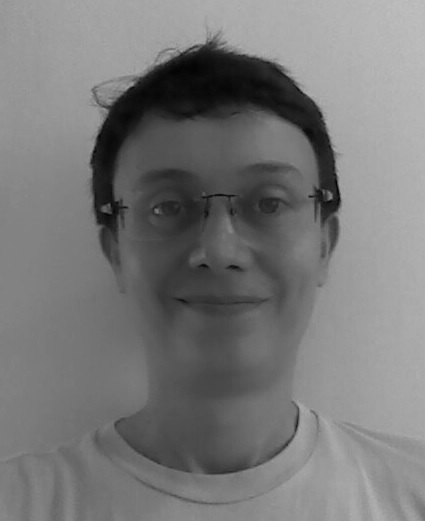
\includegraphics[width=1in,height=1.25in,clip,keepaspectratio]{alessandro3por4_2}}]{Alessandro Trindade}
received his BSc and MSc in Electrical Engineering from the Federal University of Amazonas (UFAM) in 1995 and 2015, respectively. Currently, he is pursuing his PhD in the Postgraduate Program in Informatics (PPGI) at UFAM, and holds an Assistant Professor position in the Electricity Department from UFAM. Prior to joining UFAM, he worked 4 years as Consultant of renewable energy to the Amazonas State Electric Utility and to the Inter-American Institute for Cooperation on Agriculture (IICA); he also worked for 12 years as R\&D and project manager at a non-profit foundation. His interest is in renewable energy, automated verification, and model checking.
\end{IEEEbiography}
%
%\begin{IEEEbiographynophoto}{Alessandro Trindade}
%received his BSc and MSc in Electrical Engineering from the Federal University of Amazonas (UFAM) in 1995 and 2015, respectively. Currently, he is pursuing his PhD in the Postgraduate Program in Informatics (PPGI) at UFAM, and holds an Assistant Professor position in the Electricity Department from UFAM. Prior to joining UFAM, he worked 4 years as Consultant of renewable energy to the State Electric Utility and to the Inter-American Institute for Cooperation on Agriculture (IICA); he also worked for 12 years as R\&D and project manager at a non-profit foundation (Centre of Analysis, Research and Innovation Technology Foundation). His interest is in renewable energy, automated verification, and model checking.
%\end{IEEEbiographynophoto}
%
% if you will not have a photo at all:
\begin{IEEEbiography}
    [{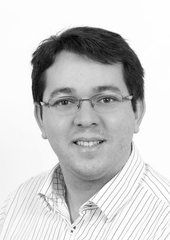
\includegraphics[width=1in,height=1.25in,clip,keepaspectratio]{lucas3por4}}]{Lucas Cordeiro}
received his Ph.D. degree in Computer Science in 2011 from the University of Southampton, UK. Currently, he is a Senior Lecturer in the School of Computer Science at the University of Manchester, and leads the Systems and Software Verification laboratory. He is also a collaborator in the Postgraduate Program in Electrical Engineering and Informatics at the Federal University of Amazonas (UFAM), Brazil. Prior to joining the University of Manchester, he worked as a researcher at Oxford University / Diffblue and as an adjunct professor at UFAM; he also worked for 4 years as software engineer at industry. His work focuses on software model checking, automated testing, program synthesis, and embedded \& cyber-physical systems.
\end{IEEEbiography}
% You can push biographies down or up by placing
% a \vfill before or after them. The appropriate
% use of \vfill depends on what kind of text is
% on the last page and whether or not the columns
% are being equalized.

%\vfill

% Can be used to pull up biographies so that the bottom of the last one
% is flush with the other column.
%\enlargethispage{-5in}



% that's all folks
\end{document}


